%!TEX root = ../Lab_report.tex
%*******************************************************************************
%*********************************** Analysis Chapter *****************************
%*******************************************************************************
\section{Free-Solution DNA electrophoresis}
Electrophoresis is an experimental technique used to separate charged molecules like polyelectrolyte chains by making use of the interaction between the particles and external electric fields. In a solution with counterions, the dynamics of a charged polymer chain is governed by electrostatic interactions between polymers and counterions as well as hydrodynamic interactions. We investigate the dynamical properties of polyelectrolytes of different lengths in a bulk solution using coarse grained Molecular Dynamics simulations with electrostatics and hydrodynamical interactions. All simulations were carried out with ESPResSo \cite{weik2019espresso}. Electrostatic interactions are modelled efficiently with the P3M method with periodic boundary conditions. The Lattice-Boltzmann method (LBM) is employed to model hydrodynamical interactions.

\subsection{System setup}
We conducted several simulations of a system with equal parameters except the number of monomers $N$ on the polyelectrolyte chain. In every simulation the system consisted of $N$ (where $1\le N \ge 32$)monomers connected by bonded interactions modelled with a FENE potential. Furthermore, $N$ counterions are placed at random positions in the simulation box. All simulated particles exhibited short ranged repulsive interactions, modelled by a WCA potential and long ranged electrostatic interactions, where a Bjerrum length of $l_\text{B} = 2.84$ in reduced units was chosen. The box size of the cubic simulation box was chosen such that the mean concentration of monomers in the solution was kept constant at $\SI{5}{\milli M}$. To remove overlap between all particles in the system, first, a total of $2000$ gradient based energy minimization steps were performed to remove overlap between all particles in the system. Subsequently, after activating electrostatic and hydrodynamic interactions, the system was equilibrated for $\SI{5e5}{}$ integration steps. During the production run, we sampled data every integration step for a total of $\SI{5e6}{}$ steps. Figure \ref{fig:vmd} displays the simulated system for one simulation with $N=32$ after equilibration.
\begin{figure}[H]
	\centering
	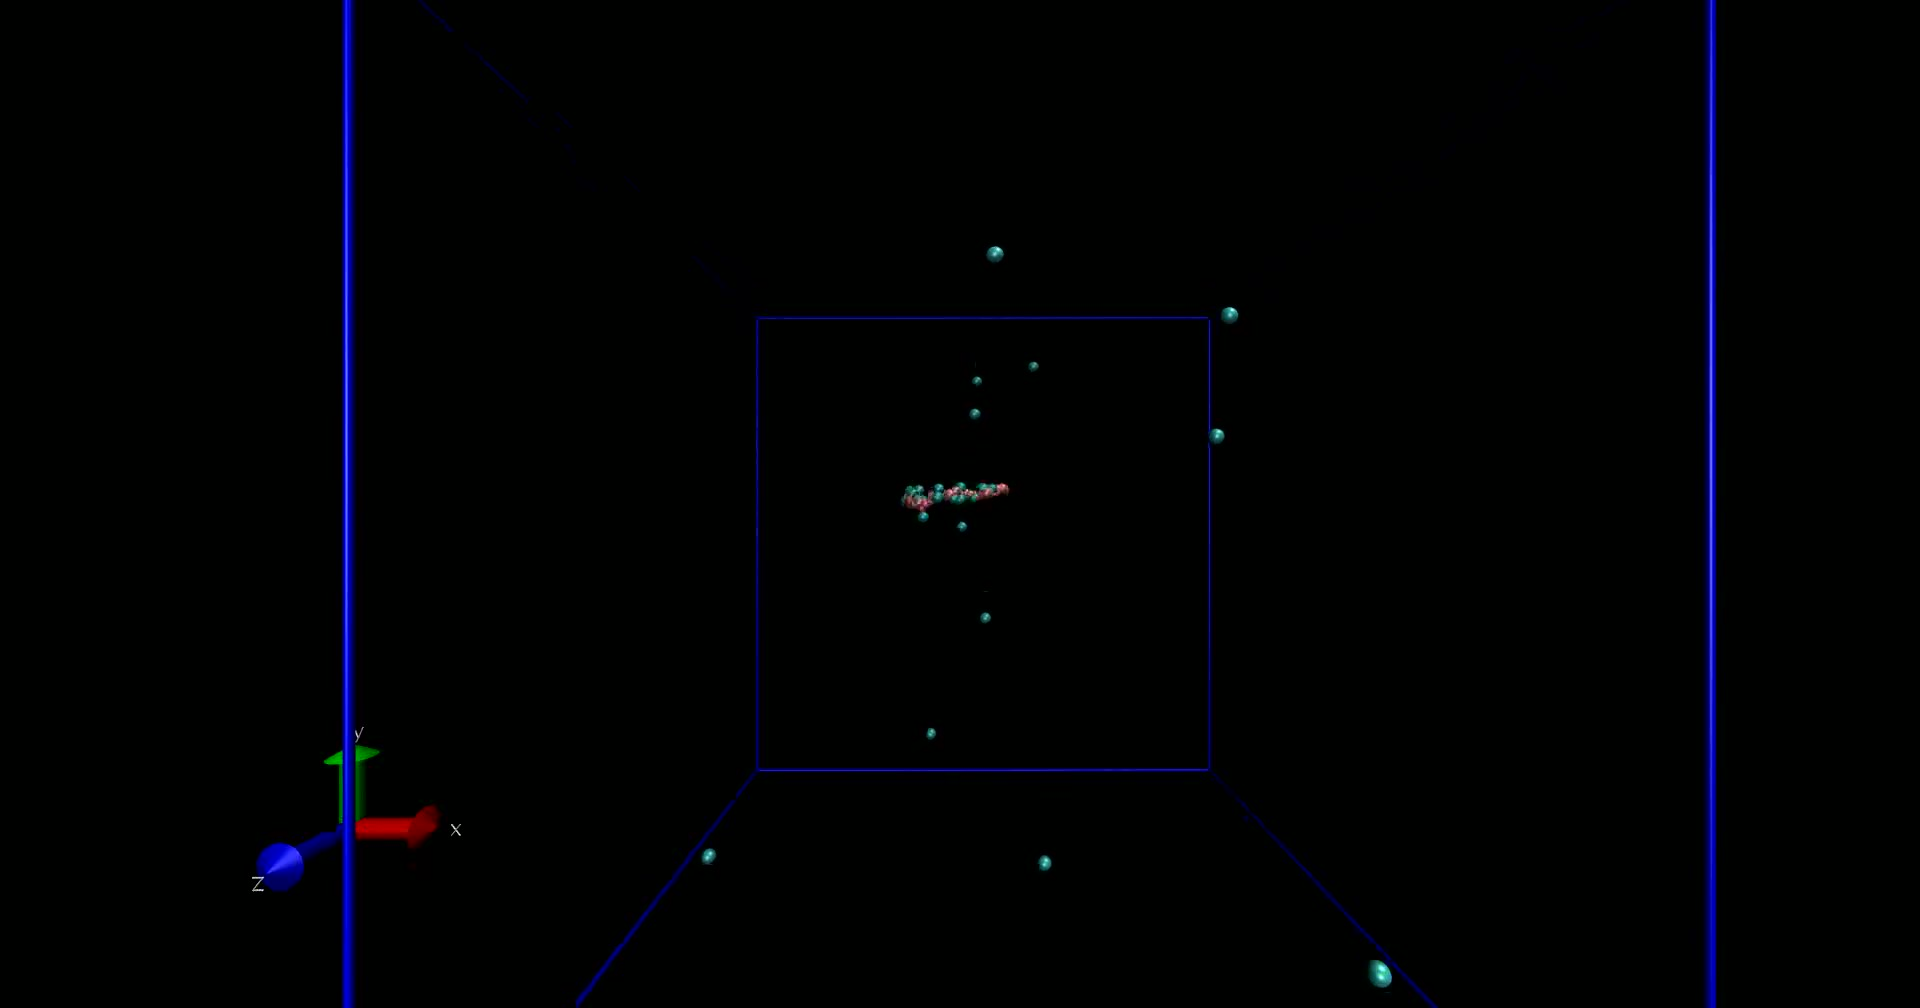
\includegraphics[width=\columnwidth]{Analysis_1/VMD_visualization}
	\captionsetup{width=\columnwidth}
	\caption{Visualization of a simulated polyelectrolyte with a chain length of 32.}
	\label{fig:vmd}
\end{figure}